In this chapter, I will shortly describe the rest of the libraries and frameworks encountered during research.

\section{SNN toolbox}
SNN toolbox (SNN-TB) \cite{rueckauerConversionContinuousValuedDeep2017} is a conversion tool which automates the process of conversion of trained ANN to an SNN. The toolbox uses a deep learning model written in one of the supported ANN frameworks (Currently Keras / TensorFlow \cite{cholletKeras15}, Lasagne \cite{sanderdielemanLasagneFirst15}, Caffe \cite{jiaCaffeConvolutional14} and PyTorch \cite{paszkePyTorchImperative19}). The provided input model is parsed and a general abstract model in Keras is derived. This internal model is used to achieve the concrete conversion to the spiking network. That is achieved by replacing the analogue neurons to spiking integrate-and-fire neurons and altering the connection weights correspondingly. The resulting spiking model can be exported to diverse spiking simulators or deployed on dedicated neuromorphic chip-sets. Currently, the supported simulation platforms are PyNN, Brian2 and built-in MegaSim and INIsim simulators. Intel Loihi and SpiNNaker project are the supported hardware platforms at the moment. Figure \ref{fig:snn-tb_workflow} illustrates the workflow of the SNN toolbox.

\begin{figure}[htbp]
    \centering
    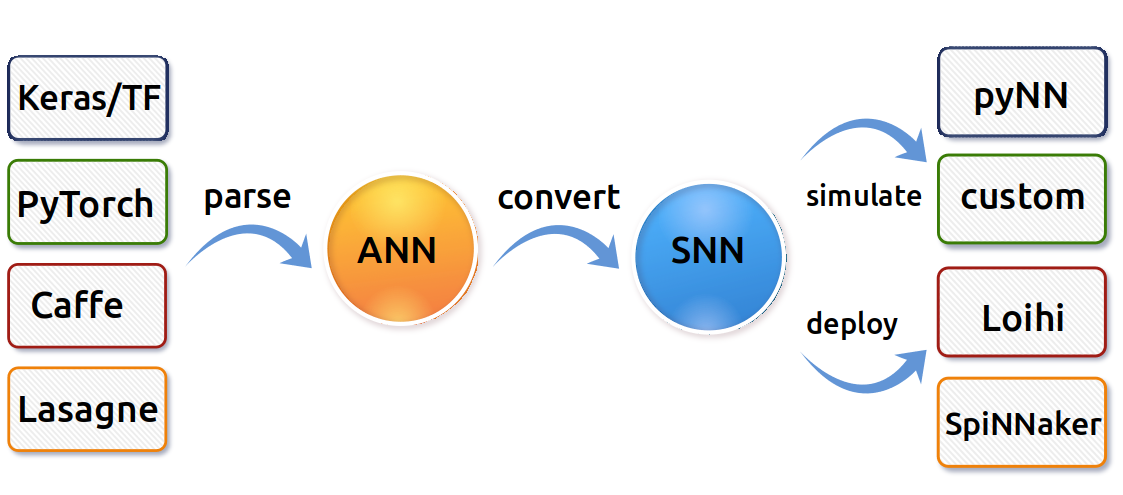
\includegraphics[width=\textwidth]{SNN-TB_workflow}
    \caption{The Illustration of the SNN toolbox workflow. An arbitrary supported deep learning model is transformed to abstract Keras model, which is subsequently converted to spiking network. Source: \url{https://snntoolbox.readthedocs.io/en/latest/guide/intro.html}}
    \label{fig:snn-tb_workflow}
\end{figure}

\section{Keras / Tensorflow}
Keras is a high-level deep learning API which can be used with multiple neural network or machine learning toolkits, mainly with TensorFlow.